
\section{Empirical Study: Are tests named for what makes them unique?}
\label{sec:unique-test-name}

Our concept-based test naming approach is based on the assumption that developers often choose the name for a test based on what aspect of the test makes the test unique among its siblings (e.g., tests in the same class).
%
To validate this assumption, we conducted an empirical study of \num{579} existing tests.
%
First, we examined each test in order to identify what makes it unique from its siblings.
%
Then we examined the test's name and judged whether the name is based either entirely or in part on the unique aspect of the test.

\subsection{Experimental Subjects}

\begin{table*}[t]
\centering
\caption{Experimental Subjects.}
\begin{tabular}
{
  l
  l
  S[table-format=5.1]
  S[table-format=5.1]
}
\toprule
\multicolumn{1}{c}{\textbf{Project}} &
\multicolumn{1}{c}{\textbf{Version}} & 
\multicolumn{1}{c}{\textbf{LoC}} &
\multicolumn{1}{c}{\textbf{\# Tests}}
\\
\midrule
 Barbecue          & 44a8632  &  10760  & 170   \\
 Guice             & 9b371d3 &  183049  & 1280   \\
 Moshi             & dbed99d  &  22168  & 716   \\
 Picasso           & a087d26  &  11006  & 229  \\
 Fastjson          & e05f1f9  &  195511  & 4950   \\
 Guava             & 368c337  &  400801  & 13962  \\
 Mockito           & 22c82dc   &  59839 & 2145   \\
 Socket.io-client  & 661f1e7  &  9478  & 85  \\
 Scribejava        & ea42bc9  &  15184  & 110   \\
 ExoPlayer         & 79da521  &  172148  & 1510   \\
 Javapoet          & e9460b8  &  10755  & 302   \\
\bottomrule
\end{tabular}
\label{tab:subjectsForStudy}
\end{table*}

To gather the tests we examined in our study, we started with the 11 Java projects shown in~\cref{tab:subjectsForStudy}.
%
In the table, the first column, Name, shows the name of the project; the second column, Version, shows the version of the project (either as a Git hash or version number) that we considered; the fourth column, LoC, shows the number of non-comment, non-blank lines of code as computed by sloc count~\cite{nguyen2007sloc}; and the final column, \# Tests, shows the number of unit tests in the project. In total, these 11 projects contain \num{25567} unit tests.

The first ten projects were randomly selected from the top \num{50} Java projects hosted on Github~\cite{top50projects}.
%
Because these projects encompass a variety of domains (e.g., JavaPoet is a library for generating Java programmatically and ExoPlayer is a media player for Android) and have many contributors (e.g., Moshi’s test suite contains contributions from \num{8} different people), their tests are more likely to be representative of tests in general which helps mitigate a potential threat to validity.
%
In addition, we also included Barbecue, a commonly used subject in the testing literature (e.g.,~\cite{zhang2015automatically, zhang2016towards,wu2020pattern}).
%
Because Barbecue is significantly smaller than the other subjects, it served as a useful starting point for the study.

Because our investigation is manual, it is necessary to reduce the \num{25567} unit tests to a more manageable number.
%
Because the projects vary widely in their numbers of tests (e.g., Guava contains \num{13962} tests while socket.io-client contains \num{85} tests), we decided to select a fixed number of tests from each project rather than choosing in proportion to test suite size.
%
This will help control for threats associated with an unbalanced sample.
%
We found that it took about \num{5} minutes to understand and code a single test.
%
Therefore we selected 40 tests from each project, giving us a total of \num{440} tests; an amount which could be analyzed in around \num{37} hours (i.e., approximately a week’s worth of effort).

When performing the selection of tests, we had an additional requirement which was to only select only tests with \enquote{good} names.
%
Prior work has demonstrated that tests often have poor names (e.g., test1, test2, etc.)~\cite{zhang2016towards}.
%
Because we are not interested in generating poor names nor understanding how poor names are chosen, it makes sense to eliminate tests with poor names from consideration.
%
Therefore, if a randomly selected test had a name that was poor it was replaced with another randomly selected test.
%
We consider a name to be poor if, with the exception of a leading \enquote{test}, the name contains only numbers (e.g., test12) or numbers and symbols (e.g., test\_2\_3).
%
We also made sure not to select any of the \num{179} tests with empty bodies contained in these applications.
%
The final set of \num{440} tests is available online: Check test names for the existence of unique parts.

\subsection{Phase 1: Discovering uniqueness of tests}

\subsubsection{Identifying what makes a test unique}

The goal of the first part of our study is to identify what makes tests unique.
%
Note that in this work we are assuming that each test has some aspect that makes it unique.
%
While we have observed cases where more than one test has the same body (i.e., duplicate tests with different names) this situation is rare, did not occur among our set of tests, and is likely indicative of a bug as there is not obvious benefit to executing the same test twice.

\subsubsection{Code creation methodology}

Identifying what makes a test unique involves comprehending not only the test under consideration but also the test’s siblings (i.e., tests that influence or restrict the name of a test).
%
In this study we consider tests declared in the same class as siblings. We chose this granularity for several reasons.
%
First, the Java programming language forbids methods with the same signature in the same class.
%
Because tests have no parameters, this means that each test in a class must have a unique name.
%
Second, tests in the same class are likely to be related (e.g., they share the same class under test).
%
This means that the aspects that make them unique are more likely to be limited in scope and therefore more interesting with respect to how tests are named.

Because there is no pre-existing classification scheme for identifying what makes a test unique, we used open, axial, and selective coding to qualitatively analyze the tests~\cite{glaser1967discovery,strauss1998basics}.
%
First, each author examined each of the \num{440} considered tests and tagged the portions of the test body that they believe are the unique aspects of the test.
%
Each tag consisted of a word or short phrase that characterizes the type of uniqueness.
%
After each author tagged each test individually, the authors together examined the tagged tests in order to reach consensus on which portion of a test’s body makes it unique and to discuss the open codes.
%
Then the authors used axial coding to establish relationships among the open codes and generated a final list of selective codes.

\subsubsection{Selective codes}

The set of selective codes is based partly on the Java language elements~\cite{chapter8class} that can comprise a test (e.g., variable declarations, method calls, control flow structures, parameters and arguments, etc).
%
However, we found that it was desirable to both refine these codes and to include other, more broad codes, in order to more precisely capture concepts that are specific to unit tests.
%
More specifically, we created four top-level codes that correspond to the high-level structure of the test (i.e., parts of test~\cite{zhang2016towards}) and multiple secondary codes that refer to test-specific elements (e.g., calls to methods of the class under test, expected or actual arguments to assertions, etc).
%
Because secondary codes refine top-level codes, they can only be applied if their corresponding top-level is applied first. Below, we discuss each top-level code and its associated secondary codes in detail.

\subsubsection{Action}

The Action code is a top-level code that is applied to a test when no sibling test shares the test’s Action - the part of the test that is the primary interaction with the application under test.

The secondary codes for the Action code relate to 
\begin{enumerate*}[label=(\roman*)]
    \item the elements of the action, specifically methods calls and arguments and
    \item whether the method calls and arguments are related to the class under test
\end{enumerate*}.
%
Because, in the context of testing, method calls to the class under test are more important than calls to methods declared by other classes and method calls in general are more important than method arguments, the secondary codes are prioritized as shown below; a lower ranked code can only be applied if no high-ranked code has been applied.
%
This ranking is based on our intuition as well as recent studies that use eye-tracking technology to understand the importance of code elements for different software engineering tasks (e.g.,\cite{rodeghero2015empirical,rodeghero2015eye,begel2018eye}).

\begin{enumerate}
    \item The CUT Method Call code is applied when 
    \begin{enumerate*}[label=(\roman*)]
        \item the test’s action contains a call to a method declared by the class under test (CUT) and
        \item no other sibling test contains a call to the same method in its action, irrespective of the method arguments
    \end{enumerate*}.
    \item The non-CUT (other) Method Call code is applied when 
    \begin{enumerate*}[label=(\roman*)]
        \item the test’s action contains a call to a method declared by a class that is not the class under test and
        \item no other sibling test contains a call to the same method in its action, irrespective of the method arguments
    \end{enumerate*}.
    \item The CUT call arguments code is applied when the test’s action contains a call to a method declared by the class under test (CUT) that has a unique set of method call arguments. 
    \item The non-CUT (other) call arguments code is applied when the test’s action contains a call to a method declared by a class that is not the class under test that has a unique set of method call arguments. 
\end{enumerate}

\subsubsection{Predicate}

The Predicate code is applied to a test when no sibling test shares the test’s predicate - the part of the test that checks the result of the performing the action.

The secondary codes for the Predicate code relate to 1) the assertions used by the test and 2) the arguments passed to the assertions.
%
Again, the secondary codes are prioritized based on their relative importance in the context of testing and a lower-ranked code can only be applied if a higher-ranked code has not already been used.

The Predicate code has noticeably more secondary codes than other top-level codes.
%
First, the definition of unit testing is to test a minimum component of a software, so the testing process is usually involved with checking the produced results.
%
Second, when checking the produced results, there are many different kinds of result-checking statements that can be used in a test, which will make the test unique.

\begin{enumerate}
    \item The actual and expected parameters code is applied when 
    \begin{enumerate*}[label=(\roman*)]
        \item the test’s predicate contains a pair of actual and expected parameters that is extracted from an assertion call and \item no other sibling test has the same pair of actual and expected parameters in its assertion calls
    \end{enumerate*}.
    \item The actual parameter code is applied when 
    \begin{enumerate*}[label=(\roman*)]
        \item the test’s predicate contains an actual parameter that is extracted from an assertion call and 
        \item no other sibling test has the same actual parameter in its assertion calls
    \end{enumerate*}.
    \item The expected parameter code is applied when 
    \begin{enumerate*}[label=(\roman*)]
        \item the test’s predicate contains an expected parameter that is extracted from an assertion call and
        \item no other sibling test has the same expected parameter in its assertion calls
    \end{enumerate*}.
    \item The assertion call code is applied when
    \begin{enumerate*}[label=(\roman*)]
        \item the test’s predicate contains an assertion call that is extracted from the assertions of the test and 
        \item no other sibling test has the same assertion call and uses it as its predicate
    \end{enumerate*}.
    \item The other result-checking call code is applied when 
    \begin{enumerate*}[label=(\roman*)]
        \item the test’s predicate contains other types of result-checking calls that serve the same functionality as JUnit assertions and 
        \item no other sibling test has the same set of result-checking calls and uses it as its predicate
    \end{enumerate*}.
    \item The only assertion code is applied when the test’s predicate contains a call to an JUnit assertion method and no other sibling test calls any JUnit assertion method (i.e., the only test with JUnit assertion).
\end{enumerate}

\subsubsection{Scenario}

The Scenario code is applied to a test when no sibling test shares the test’s scenario - the part of the test that configures or sets up the environment under which the action will be performed.

The secondary codes for the Scenario code relate to 
\begin{enumerate*}[label=(\roman*)]
    \item the elements of the scenario, specifically variable initialization and arguments in assertions, 
    \item whether the variable initialization and arguments are related to the object under test and 
    \item control flow variable and state-changing CUT call
\end{enumerate*}.
Because, in the context of testing, variable initialization to the object under test are more important than variable initialization to other objects and variable initialization in general are more important than variable initialization arguments and control flow variables.
%
And the state-changing CUT method call code is added in the list to meet the possible case of having a focal method call \cite{ghafari2015automatically}.
%
Therefore, the secondary codes are prioritized as shown below and a lower ranked code can only be applied if no high-ranked code has been applied.

\begin{enumerate}
    \item The OUT variable initialization code is applied when
    \begin{enumerate*}[label=(\roman*)]
        \item the test’s scenario contains a variable initialization that is used in a variable declaration for an object under test (OUT) and 
        \item no other sibling test contains the same variable initialization for its variable declaration for OUT and uses it as its scenario, irrespective of the arguments used in the variable initialization. The OUT variable initialization will be the tagged text, and the rest of the secondary code of the Scenario code follows the same rule (i.e., code elements are converted to the tagged text)
    \end{enumerate*}.
    \item The non-OUT (other) variable initialization code is applied when
    \begin{enumerate*}[label=(\roman*)]
        \item the test’s scenario contains a variable initialization that is used in a variable declaration but not for any object under test and 
        \item no other sibling test contains the same variable initialization for its variable declaration (i.e., not for OUT) and uses it as its scenario, irrespective of the arguments used in the variable initialization
    \end{enumerate*}.
    \item The non-OUT (other) variable initialization arguments code is applied when 
    \begin{enumerate*}[label=(\roman*)]
    \item the test’s scenario is composed of a set of arguments that are used in the variable initialization of a variable declaration but not for any object under test and
    \item no other sibling test contains the same set of arguments that are used in variable initialization of a non-OUT variable declaration and uses it as its scenario
    \end{enumerate*}.
    \item The control flow variable code is applied when 
    \begin{enumerate*}[label=(\roman*)]
        \item the test’s scenario contains a variable that is used in the conditional statement of a control flow-based statement (i.e., loop, if-else, or other type of statement) and
        \item no other sibling test contains the same variable that is used in the same type of control flow-based statement and uses it as its scenario
    \end{enumerate*}.
    \item The state-changing CUT method call code is applied when
    \begin{enumerate*}[label=(\roman*)]
        \item the test scenario is composed of a CUT method call that changes the state of the test~\cite{ghafari2015automatically} and \item no other sibling test contains the same state-changing CUT method call in its scenario, irrespective of the method arguments
    \end{enumerate*}.
\end{enumerate}

\subsubsection{Combination}

The Combination code is applied to a test when none of the other top-level codes is applicable (i.e., the test’s action, predicate, and scenario are shared with other tests).
%
The secondary codes for the Combination code enumerate the possible combinations of the first three top-level codes: Action and Predicate, Action and Scenario, Scenario and Predicate; Action, Scenario, and Predicate.
%
For example, the Action and Predicate code will be applied when the action and predicate of the tests are not unique on their own but the combination of both of them is unique among other tests in the same test class.
%
The rest of the secondary codes of the Combination code follow the same pattern. The tagged text of each secondary code of the Combination code will be the structure of the combination, such as action and predicate or action and scenario.

\subsubsection{Coding Process}

\begin{figure}[t]
\centering
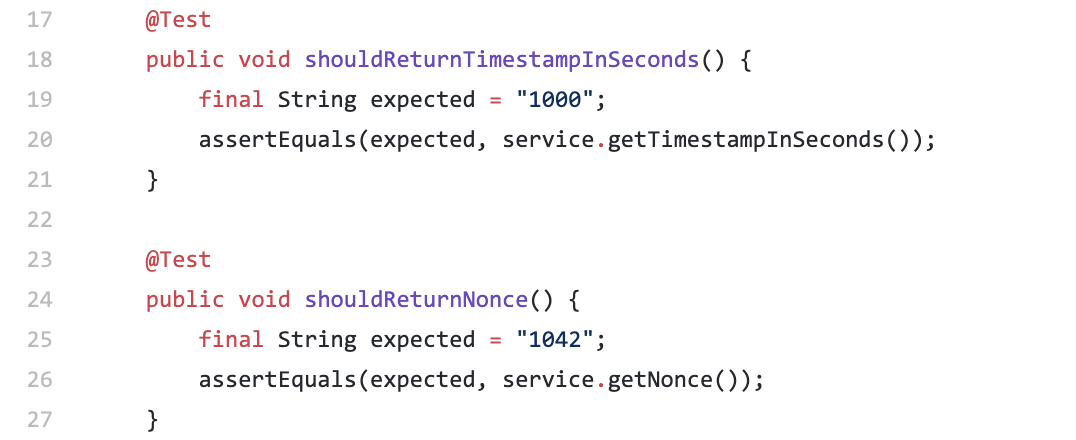
\includegraphics[scale=0.45]{figures/sp3-proposal.png}
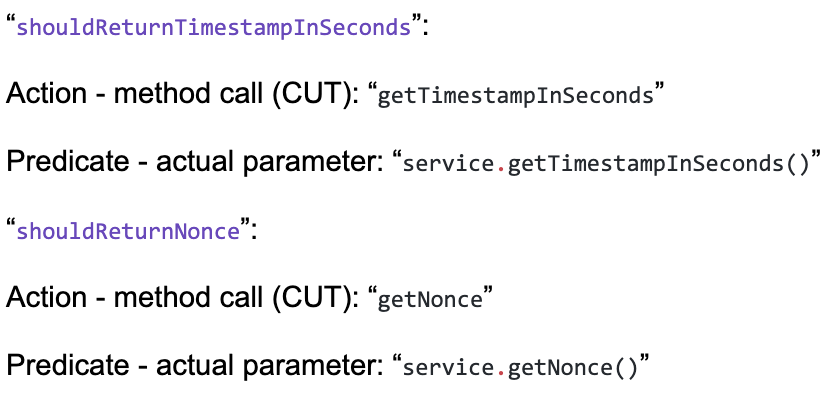
\includegraphics[scale=0.45]{figures/sp1-proposal.png}
\caption{Test cases with tagged text from the \enquote{Scribejava} project.}
\label{fig:test1-proposal}
\end{figure}

Using the selective codes and guidelines described above, each author individually recoded all of the 440 tests.
%
This was more straightforward than the initial open coding process because we were now familiar with the test and the results of the open and axial coding processes were already available.
%
Each test was first assigned one of more of the four top-level codes.  Then, for each top-level code that was assigned, one or more of the associated secondary-codes were assigned.
%
Again, after each author coded each test individually, the authors together examined the tagged tests in order to discuss and address any disagreements in the results.
%
At the end of this coding process we created a topical concordance that shows, for each code, the tests that have the corresponding type of uniqueness.
%
For the 440 tests that were selected from 11 projects, all the tagged results are shown in the online document~\cite{emp-study}. 


As an example of the selective coding process, consider the examples in~\cref{fig:test1-proposal,fig:test2-proposal}.
%
The top-half of each figure shows an excerpt of a test class from one of the subjects considered in the study.
%
Note that some minor reformatting has been done to improve the presentation (i.e., all spaces and comments are removed).
%
The bottom of each figure shows the codes applied to each test using the format: <top-level code> - <secondary code>: \enquote{<tagged text>} where <tagged text> shows the portion of the test body that is tagged by the secondary code.

\begin{figure}[t]
\centering
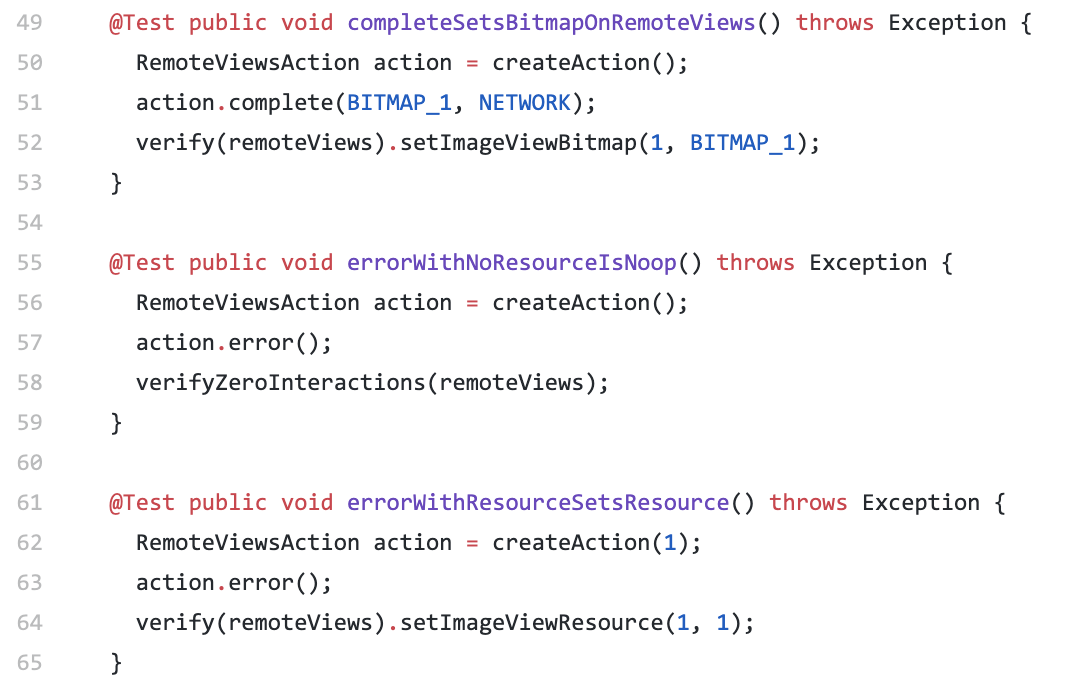
\includegraphics[scale=0.45]{figures/sp4-proposal.png}
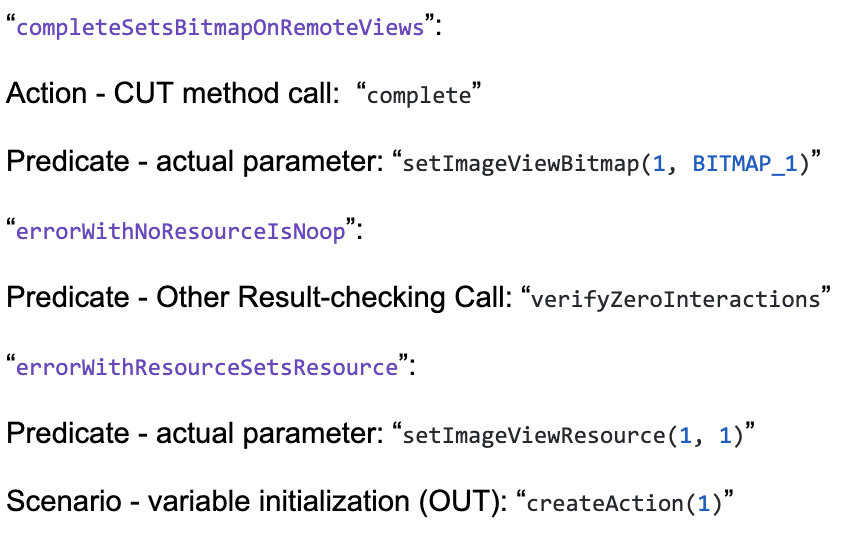
\includegraphics[scale=0.45]{figures/sp2-proposal.png}
\caption{Test cases with tagged text from the \enquote{Picasso} project.}
\label{fig:test2-proposal}
\end{figure}

For example in~\cref{fig:test1-proposal}, the test \enquote{\texttt{shouldReturnTimestampInSeconds}} is tagged with Action - method call (CUT): \enquote{\texttt{getTimestampInSeconds}} because no sibling shares the test’s action, which is to call the service’s timestamp functionality (i.e., the CUT Method \enquote{\texttt{getTimestampInSeconds()}}).
%
This test is also tagged with Predicate - actual parameter: \enquote{\texttt{service.getTimestampInSeconds()}} because no sibling test uses the result of calling \enquote{\texttt{getTimestampInSeconds}} as the actual parameter to an assertion method.
%
The test \texttt{shouldReturnNonce} is tagged with Action - CUT method call: \enquote{\texttt{getNonce}} because no sibling shares the test’s action, which is to call the service’s nonce functionality (i.e., the CUT Method \enquote{\texttt{getNonce()}}).
%
This test is also tagged with Predicate - actual parameter: \enquote{\texttt{service.getNonce()}} because no sibling test uses the result of calling \texttt{getNonce} as the actual parameter to an assertion method.

The test \texttt{shouldReturnNonce} is tagged with Action - CUT method call: \enquote{\texttt{getNonce}} because no sibling shares the test’s action, which is to call the service’s nonce functionality (i.e., the CUT Method \enquote{\texttt{getNonce()}}).
%
This test is also tagged with Predicate - actual parameter: \enquote{\texttt{service.getNonce()}} because no sibling test uses the result of calling \texttt{getNonce} as the actual parameter to an assertion method.


In~\cref{fig:test2-proposal}, the test \texttt{completeSetsBitmapOnRemoteViews} is tagged with Action - CUT method call: \enquote{\texttt{complete}} because no sibling shares the test’s action, which is to call a method to the action’s complete functionality (i.e., the CUT Method \enquote{\texttt{complete()}}).
%
This test is also tagged with Predicate - actual parameter: \enquote{\texttt{setImageViewBitmap(1, BITMAP\_1)}} because no sibling test utilizes the \texttt{setImageViewBitmap(1, BITMAP\_1)} as the actual parameter in an assertion.
%
The test \texttt{errorWithNoResourceIsNoop} is tagged with Predicate - other result-checking call: \enquote{\texttt{verifyZeroInteractions}} because no sibling shares the test’s predicate, which is to call a verification method \texttt{verifyZeroInteractions} to check the behavior of the \texttt{remoteViews} variable.
%
The test \texttt{errorWithResourceSetsResource} is tagged with Predicate - actual parameter: \enquote{\texttt{setImageViewResource(1, 1)}} because no sibling shares the test’s predicate, which is to verify the behavior of \texttt{remoteViews} variable with a specific parameter and utilizes the \texttt{setImageViewResource(1, 1)} as the actual parameter in an assertion.
%
This test is also tagged with Scenario - variable initialization (OUT): \enquote{\texttt{createAction(1)}} because no sibling shares the test’s scenario because no other test initializes the \enquote{action} variable (i.e., the object under test) using the \texttt{createAction(1)} as its variable initialization.

\subsubsection{Data and Discussion}

To better understand the results of the coding process we gathered some descriptive statistics.

\begin{table*}[t]
\centering
\caption{Data of the top-level codes.}
\begin{tabular}
{
  l
  S[table-format=5]
  S[table-format=5]
  S[table-format=5]
  S[table-format=5]
}
\toprule
\multicolumn{1}{c}{\textbf{Project}} &
\multicolumn{1}{c}{\textbf{Action}} & 
\multicolumn{1}{c}{\textbf{Predicate}} &
\multicolumn{1}{c}{\textbf{Scenario}} &
\multicolumn{1}{c}{\textbf{Combination}}
\\
 \midrule
 Barbecue          & 31  &  31   & 5     &  3 \\
 Guice             & 27  &  21   & 11    &  2 \\
 Mockito           & 23  &  25   & 18    &  3 \\
 Guava             & 20  &  19   & 11    &  5 \\
 Guice             & 23  &  23   & 24    &  1 \\
 ExoPlayer         & 26  &  21   & 10    &  4 \\
 Scribejava        & 30  &  17   & 15    &  2 \\
 Socket.io-client  & 28  &  15   & 14    &  4 \\
 Fastjson          & 30  &  26   & 7     &  3 \\
 picasso           & 16  &  24   & 10    &  2 \\
 Javapoet          & 17  &  35   & 3     &  4 \\
 \midrule
 \textbf{Sum}      & 271 &  257  & 128   &  33 \\
\bottomrule
\end{tabular}
\label{tab:top-level-codes}
\end{table*}


\begin{table*}[t]
\centering
\caption{Data for of the secondary codes.}
    \begin{subtable}[t]{1\textwidth}
    \centering
    \subcaption{Secondary codes for the Action code.}
    \begin{tabular}
    {
      l
      S[table-format=5]
      S[table-format=5.1]
    }
    \toprule
    \multicolumn{1}{c}{\textbf{Secondary Code}} &
    \multicolumn{1}{c}{\textbf{Frequency}} & 
    \multicolumn{1}{c}{\textbf{Percentage \%}}
    \\
    \midrule
     CUT call arguments     & 123  &  45.4  \\
     CUT method call        & 77   &  28.4  \\
     Other call arguments   & 44   &  16.2  \\
     Other method call      & 27   &  10.0  \\
    \bottomrule
    \end{tabular}
    \label{tab:secondary-codes-action}
    \end{subtable}
    \hfill \vspace{0.05cm}
    \begin{subtable}[t]{1\textwidth}
    \centering
    \caption{Secondary codes for the Predicate code.}
    \begin{tabular}
    {
      l
      S[table-format=5]
      S[table-format=5.1]
    }
    \toprule
    \multicolumn{1}{c}{\textbf{Secondary Code}} &
    \multicolumn{1}{c}{\textbf{Frequency}} & 
    \multicolumn{1}{c}{\textbf{Percentage \%}}
    \\
    \midrule
     Actual Parameter                & 134  &  52.1  \\
     Expected Parameter              & 78   &  30.4  \\
     Actual and Expected Parameters  & 26   &  10.1  \\
     Assertion Call                  & 18   &  7.0  \\
     Other Result-checking Call      & 1    &  0.4  \\
    \bottomrule
    \end{tabular}
    \label{tab:secondary-codes-predicate}
    \end{subtable}
    \hfill \vspace{0.05cm}
    \begin{subtable}[t]{1\textwidth}
    \centering
    \caption{Secondary codes for the Scenario code.}
    \begin{tabular}
    {
      l
      S[table-format=5]
      S[table-format=5.1]
    }
    \toprule
    \multicolumn{1}{c}{\textbf{Secondary Code}} &
    \multicolumn{1}{c}{\textbf{Frequency}} & 
    \multicolumn{1}{c}{\textbf{Percentage \%}}
    \\
    \midrule
     OUT Variable Initialization    & 94  &  73.4  \\
     Non-OUT Variable Initialization & 25   &  19.5  \\
     Non-OUT (other) Variable Initialization Arguments & 5 & 4.0  \\
     State-changing CUT Method Call       & 3   &  2.3  \\
     Control Flow Variable      & 1    &  0.8  \\
    \bottomrule
    \end{tabular}
    \label{tab:secondary-codes-scenario}
    \end{subtable}
    \hfill \vspace{0.05cm}
    \begin{subtable}[t]{1\textwidth}
    \centering
    \caption{Secondary codes for the Combination code.}
    \begin{tabular}
    {
      l
      S[table-format=5]
      S[table-format=5.1]
    }
    \toprule
    \multicolumn{1}{c}{\textbf{Secondary Code}} &
    \multicolumn{1}{c}{\textbf{Frequency}} & 
    \multicolumn{1}{c}{\textbf{Percentage \%}}
    \\
    \midrule
     action+scenario+predicate & 15   &  45.5  \\
     scenario+predicate        & 11   &  33.3  \\
     action+predicate          & 4    &  12.1  \\
     action+scenario           & 3    &  9.1  \\
    \bottomrule
    \end{tabular}
    \label{tab:secondary-codes-combination}
    \end{subtable}
\label{tab:secondary-codes}
\end{table*}

\Cref{tab:top-level-codes} shows the frequency of the top-level codes across the sampled tests.
%
In this table, the first column, Project, shows the name of the subject and the following four columns, Action through Combination, show the number of times each top-level code was applied to tests from the corresponding subject.
%
For example, the first row shows that, for the tests sampled from Barbecue, the Action code was applied \num{31} times, the Predicate code was applied \num{33} times, the Scenario code was applied \num{5} times, and the Combination code was applied \num{3} times.
%
The final row in the table shows how many times each code was applied across all tests.

\Cref{tab:secondary-codes-action,tab:secondary-codes-predicate,tab:secondary-codes-scenario,tab:secondary-codes-combination} show the frequencies of each secondary code.
%
In each table, the first column, Secondary Code, shows the secondary codes; the second column, Frequency, shows the number of times each secondary code was applied across all projects; and the final column, Percentage, shows how often the secondary code was applied, given its associated top-level code.
%
For example, the first row in Table 2a shows that the secondary code \enquote{CUT method call} was applied \num{77} times which is approximately \SI{\approx 28}{\percent} of the \num{271} times the top-level Action code was applied (i.e., when it was possible to apply the secondary code).

Based on the data shown in these tables, we can draw some general observations.
%
The first observation is about the relative frequencies of the top level codes: the Action and Predicate codes are the most common and occur about the same amount of the time (\num{271} out of \num{690}, \SI{\approx 39}{\percent} and \num{258} out of \num{690}, \SI{\approx 37}{\percent}, respectively); the Scenario code is less common (\num{128} out of \num{690}, \SI{\approx 19}{\percent}); and the Combination code is the least common and is relatively rare (\num{33} out of \num{690}, \SI{\approx 5}{\percent}).
%
This suggests that there is often a single part of a test that makes it unique among its siblings and the action and predicate are what makes it unique most often.
%
The second observation is that the relative frequencies of the top level codes within each project is largely consistent with the overall distribution.
%
With the exception of Guice, the Combination code is always the least common and the Scenario code is the second least common.
%
This suggests that the relative frequencies are likely to hold across most projects.
%
The final observation is about the relative frequencies of the secondary codes.  With the exception of the OUT Variable Initialization secondary code (\num{94} out of \num{128}, \SI{\approx 73}{\percent}), there are no dominant secondary codes (e.g., \SI{> 70}{\percent}).
%
This suggests that while there may be trends among the part of a test that makes it unique (e.g., action, scenario, and predicate), the specifics of what make each of these parts of the test unique varies greatly.
%
In addition, with the exception of the socket-io-client project (i.e., it relies on the secondary codes under the action and predicate top-level codes, 43 out of 61, \SI{\approx 70.5}{\percent}), there are also no dominant secondary codes (e.g., \SI{> 70}{\percent}) at the project level, and the rest of the detailed data can be found in the online document~\cite{emp-study}.

\subsection{Phase 2: Deciding whether unit tests are named after what makes them unique}

The goal of the second part of our study is to investigate whether tests are named, either wholly or in part, after what makes them unique.
%
In order to decide whether tests are named after what makes them unique, we proposed two research questions:
\begin{itemize}
    \item RQ1: Is uniqueness used as a naming rationale for JUnit tests?
    \item RQ2: When uniqueness is the naming rationale, does the tagged text appear directly in the name or is it transformed?
\end{itemize}

\subsubsection{RQ1: Is uniqueness used as a naming rationale in JUnit tests?}

To investigate RQ1, we manually compared the name of each test against the aspects that make it unique which were identified in the first part of the study.
%
The comparison between the test name and tagged text (i.e.,the aspects of the test that make it unique) is performed as follows.
%
First, we manually split the test names and the tagged text into a set of tokens, and the splitting of the names is based on a customized tokenizer for software analysis~\cite{enslen2009mining}.
%
Then we remove the leading \enquote{text} and lower case all tokens. For example, the test name \texttt{testPostReturnsBarcodeImage} is parsed into a set of tokens: \enquote{[post, returns, barcode, image]}.
%
Finally, we manually compared the two sets of tokens. Each author did this comparison individually and classified the tests into one of the following categories based on the degree to which the name appears to be based on the tagged text.

\begin{table*}[t]
\centering
\caption{Results to check if the tokens are identical or transformed.}
\begin{tabular}
{
  l
  S[table-format=5]
  S[table-format=5]
  S[table-format=5]
  S[table-format=5]
  S[table-format=5]
  S[table-format=5]
  S[table-format=5]
}
\toprule
\multicolumn{1}{c}{\textbf{Project}} & \multicolumn{3}{c}{\textbf{Full}} & \multicolumn{3}{c}{\textbf{Partial}} & \multicolumn{1}{c}{\textbf{None}}\\
\cmidrule(lr){2-4}
\cmidrule(lr){5-7}
\cmidrule(lr){8-8}

& \multicolumn{1}{c}{\textbf{Identical}} & \multicolumn{1}{c}{\textbf{Transformed}} & 
\multicolumn{1}{c}{\textbf{Total \#}} &
\multicolumn{1}{c}{\textbf{Identical}} &
\multicolumn{1}{c}{\textbf{Transformed}} &
\multicolumn{1}{c}{\textbf{Total \#}} &
\multicolumn{1}{c}{\textbf{Total \#}}
\\
\midrule
 Barbecue           & 2  &  0  & 2   & 32 & 27 & 5 & 6 \\
 Moshi              & 5 &  5  & 0   & 18 & 16 & 2 & 17 \\
 Mockito            & 4  &  3  & 1   & 27 & 24 & 3 & 9 \\
 Guava              & 2  &  2  & 0  & 30 & 27 & 3 & 8 \\
 Guice              & 1  &  1  & 0   & 36 & 29 & 7 & 3 \\
 ExoPlayer          & 3  &  3  & 0  & 19 & 16 & 3 & 18 \\
 Scribejava         & 5  &  5  & 0  & 31 & 28 & 3 & 4 \\
 Socket.io-client   & 0  &  0  & 0  & 36 & 22 & 14 & 4 \\
 Fastjson           & 1  &  1  & 0   & 20 & 19 & 1 & 19 \\
 Picasso            & 2  &  2  & 0   & 29 & 25 & 4 & 9 \\
 Javapoet           & 0  &  0  & 0   & 31 & 28 & 3 & 9 \\
 \midrule
 Overall            & 25 &  22  &  3  & 309 & 261 & 48 & 106 \\
\bottomrule
\end{tabular}
\label{tab:identical-or-transformed.}
\end{table*}



